% This is the template used for the GIH thesis. It is based on 
% Reed College LaTeX thesis template. Most of the work (Reed template)
% for the document class was done by Sam Noble (SN), as well as this
% template. Later comments etc. by Ben Salzberg (BTS). Additional
% restructuring and APA support by Jess Youngberg (JY).
%
% See http://web.reed.edu/cis/help/latex.html for help. There are a
% great bunch of help pages there, with notes on
% getting started, bibtex, etc. Go there and read it if you're not
% already familiar with LaTeX.
%
% Any line that starts with a percent symbol is a comment.
% They won't show up in the document, and are useful for notes
% to yourself and explaining commands.
% Commenting also removes a line from the document;
% very handy for troubleshooting problems. -BTS

% The template was updated by Daniel Hammarström to fit GIH
% requirements. Additional code was borrowed from the 
% Stockholm University (Andreas Solders 2011) template.

% The template was forked from the thesisdown package (CII updates)

%%
%% Preamble
%%
% \documentclass{<something>} must begin each LaTeX document
\documentclass[twoside,10pt]{gihclass} %Default style using S5 paper
% Packages are extensions to the basic LaTeX functions. Whatever you
% want to typeset, there is probably a package out there for it.
% Chemistry (chemtex), screenplays, you name it.
% Check out CTAN to see: http://www.ctan.org/
%%
\usepackage{graphicx,latexsym}
\usepackage{amsmath}
\usepackage{amssymb,amsthm}
\usepackage{longtable,booktabs,setspace}
\usepackage{chemarr} %% Useful for one reaction arrow, useless if you're not a chem major
\usepackage[hyphens]{url}
% Added by CII
\usepackage{hyperref,xcolor}
\hypersetup{
    colorlinks = false,
    pdfborder={0 0 0}
}
\usepackage{lmodern}
\usepackage{float}
\floatplacement{figure}{H}
% End of CII addition
\usepackage{rotating}

% Next line commented out by CII
%%% \usepackage{natbib}
% Comment out the natbib line above and uncomment the following two lines to use the new
% biblatex-chicago style, for Chicago A. Also make some changes at the end where the
% bibliography is included.
%\usepackage{biblatex-chicago}
%\bibliography{thesis}


% Added by CII (Thanks, Hadley!)
% Use ref for internal links
\renewcommand{\hyperref}[2][???]{\autoref{#1}}
\def\chapterautorefname{Chapter}
\def\sectionautorefname{Section}
\def\subsectionautorefname{Subsection}
% End of CII addition

% Added by CII
\usepackage{caption}
\captionsetup{width=5in}
% End of CII addition


% \usepackage{times} % other fonts are available like times, bookman, charter, palatino


% Syntax highlighting #22

% To pass between YAML and LaTeX the dollar signs are added by CII

% New variables 2019-02-06 GIH copyright info 
\isbn{Provided by the library} 
\place{Stockholm}
\printeby{Printer service, Stockholm, 2019}
\coverinfo{}
\year{2019}



\title{Determinants of intra-individual variation in adaptability to resistance training of different volumes with special reference to skeletal muscle phenotypes}
\author{Daniel Hammarström}
% The month and year that you submit your FINAL draft TO THE LIBRARY (May or December)
\date{May 20xx}


%If you have two advisors for some reason, you can use the following
% Uncommented out by CII
\sernr{999}
% End of CII addition
%%% Remember to use the correct department!

% if you're writing a thesis in an interdisciplinary major,
% uncomment the line below and change the text as appropriate.
% check the Senior Handbook if unsure.
%\thedivisionof{The Established Interdisciplinary Committee for}
% if you want the approval page to say "Approved for the Committee",
% uncomment the next line
%\approvedforthe{Committee}

% Added by CII
%%% Copied from knitr
%% maxwidth is the original width if it's less than linewidth
%% otherwise use linewidth (to make sure the graphics do not exceed the margin)
\makeatletter
\def\maxwidth{ %
  \ifdim\Gin@nat@width>\linewidth
    \linewidth
  \else
    \Gin@nat@width
  \fi
}
\makeatother

\renewcommand{\contentsname}{Table of Contents}
% End of CII addition

\setlength{\parskip}{0pt}

% Added by CII

\providecommand{\tightlist}{%
  \setlength{\itemsep}{0pt}\setlength{\parskip}{0pt}}




\Dedication{
You can have a dedication here if you wish.
}

\Preface{

}

\Abstract{
The preface pretty much says it all.

\par

Second paragraph of abstract starts here.
}

\Listofpapers{
\begin{enumerate}
\def\labelenumi{\Roman{enumi}.}
\item
  \textbf{Hammarström D}, Øfsteng S, Koll L, Hanestadhaugen M, Hollan I, Apró W, Blomstrand E, Rønnestad B, Ellefsen S Benefits of higher resistance-training volume are related to ribosome biogenesis. The \emph{Journal of physiology}. 2020 Feb;598(3):543-565. doi: 10.1113/JP278455.
\item
  Khan Y, \textbf{Hammarström D}, Rønnestad B, Ellefsen S, Ahmad R Increased biological relevance of transcriptome analyses in human skeletal muscle using a model-specific pipeline. \emph{BMC Bioinformatics}. 2020 Nov 30;21(1):548. doi: 10.1186/s12859-020-03866-y
\item
  \textbf{Hammarström D}, Øfsteng S, Jacobsen N, Flobergseter K, Rønnestad B, Ellefsen S Ribosome accumulation during early phase resistance training. \emph{Manuscript}
\end{enumerate}
}


	\usepackage{lettrine} \usepackage{booktabs} \usepackage{longtable} \usepackage{array} \usepackage{multirow} \usepackage{wrapfig} \usepackage{float} \usepackage{colortbl} \usepackage{pdflscape} \usepackage{tabu} \usepackage{threeparttable} \usepackage{threeparttablex} \usepackage[normalem]{ulem} \usepackage{makecell} \usepackage{siunitx}
	\usepackage{booktabs}
 \usepackage{longtable}
 \usepackage{array}
 \usepackage{multirow}
 \usepackage{wrapfig}
 \usepackage{float}
 \usepackage{colortbl}
 \usepackage{pdflscape}
 \usepackage{tabu}
 \usepackage{threeparttable}
 \usepackage{threeparttablex}
 \usepackage[normalem]{ulem}
 \usepackage{makecell}
% End of CII addition
%%
%% End Preamble
%%
%


% Added updated related to csl update in Pandoc
\newlength{\cslhangindent}
\setlength{\cslhangindent}{1.5em}
\newlength{\csllabelwidth}
\setlength{\csllabelwidth}{3em}
\newenvironment{CSLReferences}[3] % #1 hanging-ident, #2 entry spacing
 {% don't indent paragraphs
  \setlength{\parindent}{0pt}
  % turn on hanging indent if param 1 is 1
  \ifodd #1 \everypar{\setlength{\hangindent}{\cslhangindent}}\ignorespaces\fi
  % set entry spacing
  \ifnum #2 > 0
  \setlength{\parskip}{#2\baselineskip}
  \fi
 }%
 {}
\usepackage{calc} % for \widthof, \maxof
\newcommand{\CSLBlock}[1]{#1\hfill\break}
\newcommand{\CSLLeftMargin}[1]{\parbox[t]{\maxof{\widthof{#1}}{\csllabelwidth}}{#1}}
\newcommand{\CSLRightInline}[1]{\parbox[t]{\linewidth}{#1}}
\newcommand{\CSLIndent}[1]{\hspace{\cslhangindent}#1}


\begin{document}




% Everything below added by CII


\frontmatter % this stuff will be roman-numbered
% \pagestyle{empty} % this removes page numbers from the frontmatter
  \maketitle
  \begin{dedication}
  \topskip0pt
\vspace*{\fill}
 You can have a dedication here if you wish.
\vspace*{\fill}
  \end{dedication}
\begin{defence}
    THESIS FOR DOCTORAL DEGREE (Ph.D.)\\
    ~\\
    ~\\
    \textbf{The title of your thesis}\\
    ~\\
    by\\
    \textbf{Your name}\\
    ~\\
    ~\\
    Thesis for Philosophy of Doctoral Degree in Sport Sciences, at The Swedish School of Sport and Health Sciences (GIH), which, according to the decision of the dean, will be publicly defended on \emph{DATE}. The thesis defense will be held at the auditorium at The Swedish School of Sport and Health Sciences (GIH), Stockholm.\\
    ~\\
    ~\\
    \textbf{Opponent}\\
    Profesor \ldots.\\
    ~\\
    \textbf{Principal supervisor}\\
    Profesor\ldots{}\\
    ~\\
    \textbf{Co-supervisor(s)}\\
    -Professor\ldots{}\\
    -Professor\ldots{}\\
    -Professor\ldots{}\\
    ~\\
    \textbf{Examination board}\\
    -Associate professor\ldots{}\\
    -Professor \ldots{}\\
    -Professor \ldots{}
  \end{defence}

  \begin{abstract}
    The preface pretty much says it all.

    \par

    Second paragraph of abstract starts here.
  \end{abstract}
  \begin{listofpapers}
    \begin{enumerate}
    \def\labelenumi{\Roman{enumi}.}
    \item
      \textbf{Hammarström D}, Øfsteng S, Koll L, Hanestadhaugen M, Hollan I, Apró W, Blomstrand E, Rønnestad B, Ellefsen S Benefits of higher resistance-training volume are related to ribosome biogenesis. The \emph{Journal of physiology}. 2020 Feb;598(3):543-565. doi: 10.1113/JP278455.
    \item
      Khan Y, \textbf{Hammarström D}, Rønnestad B, Ellefsen S, Ahmad R Increased biological relevance of transcriptome analyses in human skeletal muscle using a model-specific pipeline. \emph{BMC Bioinformatics}. 2020 Nov 30;21(1):548. doi: 10.1186/s12859-020-03866-y
    \item
      \textbf{Hammarström D}, Øfsteng S, Jacobsen N, Flobergseter K, Rønnestad B, Ellefsen S Ribosome accumulation during early phase resistance training. \emph{Manuscript}
    \end{enumerate}
  \end{listofpapers}

  \hypersetup{linkcolor=black}
  \setcounter{tocdepth}{2}
  \tableofcontents

  \listoftables

  \listoffigures




\mainmatter % here the regular arabic numbering starts
\pagestyle{fancyplain} % turns page numbering back on

\hypertarget{thesisdownthesis_gitbook-default}{%
\chapter{thesisdown::thesis\_gitbook: default}\label{thesisdownthesis_gitbook-default}}

Placeholder

\hypertarget{background}{%
\chapter{Background}\label{background}}

Placeholder

\hypertarget{resistance-exercise-prescription-influences-and-challenges}{%
\section{Resistance-exercise prescription, influences and challenges}\label{resistance-exercise-prescription-influences-and-challenges}}

\hypertarget{adaptations-to-resistance-training}{%
\section{Adaptations to resistance training}\label{adaptations-to-resistance-training}}

\hypertarget{muscle-hypertrophy-and-strength}{%
\subsection{Muscle hypertrophy and strength}\label{muscle-hypertrophy-and-strength}}

\hypertarget{changes-in-muscle-fiber-contractile-and-metabolic-characteristics-with-resistance-training}{%
\subsection{Changes in muscle fiber contractile and metabolic characteristics with resistance training}\label{changes-in-muscle-fiber-contractile-and-metabolic-characteristics-with-resistance-training}}

\hypertarget{connective-tissue}{%
\subsection{Connective tissue}\label{connective-tissue}}

\hypertarget{effects-of-exercise-prescription-on-muscle-mass-and-strength}{%
\section{Effects of exercise prescription on muscle mass and strength}\label{effects-of-exercise-prescription-on-muscle-mass-and-strength}}

\hypertarget{effects-of-resistance-exercise-volume-on-muscle-strength-and-mass}{%
\subsection{Effects of resistance exercise volume on muscle strength and mass}\label{effects-of-resistance-exercise-volume-on-muscle-strength-and-mass}}

\hypertarget{molecular-determinants-of-training-induced-muscle-hypertrophy}{%
\section{Molecular determinants of training-induced muscle hypertrophy}\label{molecular-determinants-of-training-induced-muscle-hypertrophy}}

\hypertarget{mtor}{%
\subsection{mTOR}\label{mtor}}

\hypertarget{ribosomal-biogenesis}{%
\subsection{Ribosomal biogenesis}\label{ribosomal-biogenesis}}

\hypertarget{transcriptional-regulation-of-muscle-mass}{%
\subsection{Transcriptional regulation of muscle mass}\label{transcriptional-regulation-of-muscle-mass}}

\hypertarget{ribosomal-biogensis-as-a-determinant-of-rt-induced-hypertrophy}{%
\subsubsection{Ribosomal biogensis as a determinant of RT-induced hypertrophy}\label{ribosomal-biogensis-as-a-determinant-of-rt-induced-hypertrophy}}

\hypertarget{protein-synthesis}{%
\subsection{Protein synthesis}\label{protein-synthesis}}

\hypertarget{the-mammalian-target-of-rapamycin-mtor-and-translational-efficiency}{%
\subsection{The mammalian target of rapamycin (mTOR) and translational efficiency}\label{the-mammalian-target-of-rapamycin-mtor-and-translational-efficiency}}

\hypertarget{ribsome-biogenesisand-muscle-growth}{%
\section{Ribsome biogenesisand muscle growth}\label{ribsome-biogenesisand-muscle-growth}}

\hypertarget{effects-of-exercise-volume-on-molecular-determinants-of-muscle-growth}{%
\section{Effects of exercise volume on molecular determinants of muscle growth}\label{effects-of-exercise-volume-on-molecular-determinants-of-muscle-growth}}

\hypertarget{from-training-response}{%
\subsection{From Training response}\label{from-training-response}}

\hypertarget{from-rna-seq}{%
\section{From RNA-seq}\label{from-rna-seq}}

\hypertarget{from-tr10}{%
\section{From tr10}\label{from-tr10}}

\hypertarget{aims}{%
\chapter{Aims}\label{aims}}

The primary aim of this thesis was to relate the adaptive response to resistance training with low- and moderate-volume to skeletal-muscle characteristics in previously untrained individuals. The key question was whether manipulation of exercise-volume will have diverse effects in different individuals related to muscular intrinsic characteristics. A further aim was to characterize exercise-volume dependence in muscle molecular characteristics and determine a time course profile of markers of ribosomal biogenesis in response to resistance training. Based on these aims, the objectives of the present thesis were;
\begin{itemize}
\tightlist
\item
  to relate skeletal muscle and systemic characteristics to benefit of moderate- compared to low-volume resistance training;
\item
  To determine volume-dependence in molecular networks related to muscle growth and remodeling in response to resistance training
\item
  To determine a time course of markers related to ribosome biogenesis in the early phase of resistance training.
\end{itemize}
\hypertarget{methods}{%
\chapter{Methods}\label{methods}}

Placeholder

\hypertarget{study-protocols-and-participants}{%
\section{Study protocols and participants}\label{study-protocols-and-participants}}

\hypertarget{resistance-training-interventions}{%
\section{Resistance training interventions}\label{resistance-training-interventions}}

\hypertarget{muscle-strength-assessments}{%
\section{Muscle strength assessments}\label{muscle-strength-assessments}}

\hypertarget{isokinetic-and-isometric-maximal-torque}{%
\subsection{Isokinetic and isometric maximal torque}\label{isokinetic-and-isometric-maximal-torque}}

\hypertarget{one-repetition-maximum}{%
\subsection{One-repetition maximum}\label{one-repetition-maximum}}

\hypertarget{strength-assessment-frequency-and-statistics}{%
\subsection{Strength assessment frequency (and statistics)}\label{strength-assessment-frequency-and-statistics}}

\hypertarget{measures-of-muscle-mass}{%
\section{Measures of muscle mass}\label{measures-of-muscle-mass}}

\hypertarget{muscle-tissue-sampling-and-preparations-for-downstream-analyses}{%
\section{Muscle tissue sampling and preparations for downstream analyses}\label{muscle-tissue-sampling-and-preparations-for-downstream-analyses}}

\hypertarget{total-rna-extraction}{%
\subsubsection{Total RNA extraction}\label{total-rna-extraction}}

\hypertarget{protein-extraction-immunoblotting}{%
\subsubsection{Protein extraction immunoblotting}\label{protein-extraction-immunoblotting}}

\hypertarget{rna-analysis}{%
\section{RNA analysis}\label{rna-analysis}}

\hypertarget{hormonal-measurements}{%
\subsection{Hormonal measurements}\label{hormonal-measurements}}

\hypertarget{statistics-and-data-analysis}{%
\section{Statistics and data analysis}\label{statistics-and-data-analysis}}

\hypertarget{normalization}{%
\subsection{Normalization}\label{normalization}}

\hypertarget{meta-analysis-of-within-session-training-volume}{%
\section{Meta-analysis of within-session training volume}\label{meta-analysis-of-within-session-training-volume}}

\hypertarget{literature-search-inclusion-criteria-and-coding-of-studies}{%
\subsection{Literature search, inclusion criteria and coding of studies}\label{literature-search-inclusion-criteria-and-coding-of-studies}}

\hypertarget{calculations-of-effect-sizes-and-statistical-analysis}{%
\subsection{Calculations of effect sizes and statistical analysis}\label{calculations-of-effect-sizes-and-statistical-analysis}}

\hypertarget{results-and-discussion}{%
\chapter{Results and Discussion}\label{results-and-discussion}}

\hypertarget{effects-of-different-training-volume-on-changes-in-muscle-size-and-function}{%
\section{Effects of different training volume on changes in muscle size and function}\label{effects-of-different-training-volume-on-changes-in-muscle-size-and-function}}

In Study I, the average increases in muscle strength and mass in each volume condition corresponded to what could be expected based on previous research in young healthy participants (Table \ref{tab:csa-str-tab})
{[}1, 2{]},
indicating the general efficiency of the training program.




\begin{table}

\caption{\label{tab:csa-str-tab}Training induced changes in muscle CSA and average strength in Study I}
\centering
\fontsize{7}{9}\selectfont
\begin{tabular}[t]{lllll}
\toprule
 & Sex & Volume condition & Mean (SD) & Reference\\
\midrule
 &  & LOW & 3.05 (3.61) & \\
\cmidrule{3-4}
 & \multirow{-2}{*}{\raggedright\arraybackslash Female} & MOD & 5.02 (4.04) & \\
\cmidrule{2-4}
 &  & LOW & 3.83 (3.50) & \\
\cmidrule{3-4}
\multirow{-4}{*}{\raggedright\arraybackslash CSA \%-change} & \multirow{-2}{*}{\raggedright\arraybackslash Male} & MOD & 5.10 (3.71) & \multirow{-4}{*}{\raggedright\arraybackslash }\\
\cmidrule{1-5}
 &  & LOW & 0.04 (0.05) & \\
\cmidrule{3-4}
 & \multirow{-2}{*}{\raggedright\arraybackslash Female} & MOD & 0.07 (0.05) & \\
\cmidrule{2-4}
 &  & LOW & 0.05 (0.05) & \\
\cmidrule{3-4}
\multirow{-4}{*}{\raggedright\arraybackslash CSA \%-change per day} & \multirow{-2}{*}{\raggedright\arraybackslash Male} & MOD & 0.07 (0.05) & \multirow{-4}{*}{\raggedright\arraybackslash 0.11 [0.04-0.26]a}\\
\cmidrule{1-5}
 &  & LOW & 0.11 (0.13) & \\
\cmidrule{3-4}
 & \multirow{-2}{*}{\raggedright\arraybackslash Female} & MOD & 0.18 (0.15) & \multirow{-2}{*}{\raggedright\arraybackslash 0.08 (0.22)b}\\
\cmidrule{2-5}
 &  & LOW & 0.14 (0.12) & \\
\cmidrule{3-4}
\multirow{-4}{*}{\raggedright\arraybackslash CSA \%-change per session} & \multirow{-2}{*}{\raggedright\arraybackslash Male} & MOD & 0.19 (0.13) & \multirow{-2}{*}{\raggedright\arraybackslash 0.14 (0.14)b}\\
\cmidrule{1-5}
 &  & LOW & 21.0 (9.8) & \\
\cmidrule{3-4}
 & \multirow{-2}{*}{\raggedright\arraybackslash Female} & MOD & 27.8 (14.4) & \\
\cmidrule{2-4}
 &  & LOW & 19.2 (12.4) & \\
\cmidrule{3-4}
\multirow{-4}{*}{\raggedright\arraybackslash Average strength \%-change} & \multirow{-2}{*}{\raggedright\arraybackslash Male} & MOD & 23.1 (12.0) & \multirow{-4}{*}{\raggedright\arraybackslash }\\
\cmidrule{1-5}
 &  & LOW & 0.77 (0.36) & \\
\cmidrule{3-4}
 & \multirow{-2}{*}{\raggedright\arraybackslash Female} & MOD & 1.00 (0.49) & \multirow{-2}{*}{\raggedright\arraybackslash 0.67 (0.35)b}\\
\cmidrule{2-5}
 &  & LOW & 0.72 (0.48) & \\
\cmidrule{3-4}
\multirow{-4}{*}{\raggedright\arraybackslash Average strength \%-change per session} & \multirow{-2}{*}{\raggedright\arraybackslash Male} & MOD & 0.87 (0.46) & \multirow{-2}{*}{\raggedright\arraybackslash 0.47 (0.22)b}\\
\bottomrule
\multicolumn{5}{l}{\textsuperscript{a} Estimates from Wernbom et al. {[}1{]}}\\
\multicolumn{5}{l}{\textsuperscript{b} Estimates from Ahtiainen et al. {[}2{]}}\\
\end{tabular}
\end{table}
The moderate-volume condition consistently showed favorable adaptations when compared to the low-volume condition in measures of muscle hypertrophy and strength gains (Figure \ref{fig:comb-fig-s1}).
In an attempt to explain differences in training outcomes between volume-conditions, selected molecular markers with known influence on adaptations to resistance training were investigated for volume-dependency.
First, activation of signaling along the mechanosensitive mTORC1-pathway has previously been shown to correlate with training-induced muscle growth
{[}3, 4, 5{]}.
A commonly used readout of mTORC1-signaling is the phosphorylation of S6-kinase (S6K1) at Thr\textsuperscript{389}/Thr\textsuperscript{412} which in turn preceeds phosphorylation of ribosomal protein S6. In the present study S6K1\textsuperscript{Thr\textsuperscript{389}/Thr\textsuperscript{412}}

Given these limitations in using mTORC-signalling as markers of muscle hypertrophy, it is not surprising that previous studies are ambiguous in their associative approach between acute mTORC1-related phosphorylation and hypertrophy in humans. Some studies find a strong correlation

{[}6, 7{]}.

{[}8{]};
{[}4{]};

This seems somewhat counterintuitive, as this pathway is a known regulator of translation initiation and elongation, as well as of ribosomal biogenesis
{[}9, 10,\\
11, 12{]}

Indeed, in the present study we observed volume-dependence of mTOR phosphorylation at Ser2448, which could be a sign of negative feedback from mTORC1-based activation of S6K1 {[}13{]}.
{[}14{]};
{[}15{]};
{[}16{]}{]}.
Furthermore, when a combining data from more recent studies indicates that a higher training volume is generally associated with increased muscle hypertrophy and strength gains (Figure \ref{fig:comb-fig-s1} and \ref{fig:comb-fig-s1}.

In Study II, training efficacy was assessed by comparing outcomes to a non-training control group. The training group displayed increases compared to the control group for both strength muscle thickness measures.
\begin{figure}

{\centering 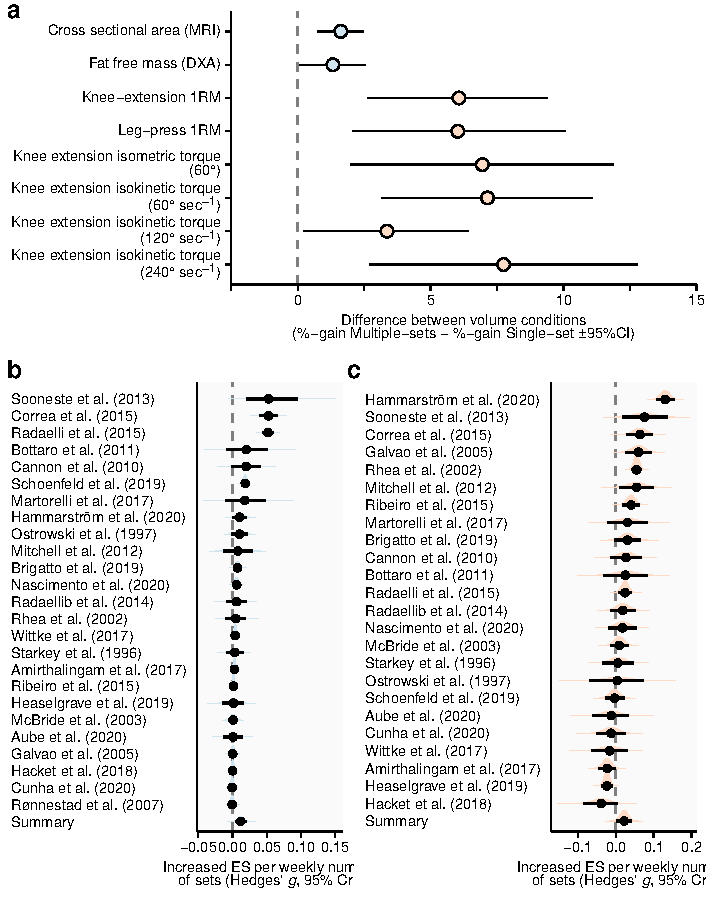
\includegraphics{thesis_files/figure-latex/comb-fig-s1-1} 

}

\caption[Differences in training induced changes to muscle mass and strength measures between volume conditions in Study I]{Differences in training induced relative changes in muscle mass and strength measures. Estimates are derived from ANCOVA models controling for baseline values and sex.}\label{fig:comb-fig-s1}
\end{figure}
\hypertarget{acute-effects-of-diffrent-training-volume-on-determinants-of-muscle-protein-synthesis}{%
\section{Acute effects of diffrent training volume on determinants of muscle protein synthesis}\label{acute-effects-of-diffrent-training-volume-on-determinants-of-muscle-protein-synthesis}}

\hypertarget{general-discussion}{%
\chapter{General Discussion}\label{general-discussion}}

\hypertarget{conclusion}{%
\chapter*{Conclusion}\label{conclusion}}
\addcontentsline{toc}{chapter}{Conclusion}

If we don't want Conclusion to have a chapter number next to it, we can add the \texttt{\{-\}} attribute.

\textbf{More info}

And here's some other random info: the first paragraph after a chapter title or section head \emph{shouldn't be} indented, because indents are to tell the reader that you're starting a new paragraph. Since that's obvious after a chapter or section title, proper typesetting doesn't add an indent there.

\hypertarget{references}{%
\chapter*{References}\label{references}}
\addcontentsline{toc}{chapter}{References}

Placeholder

\hypertarget{refs}{}
\begin{CSLReferences}{0}{0}
\leavevmode\hypertarget{ref-RN2007}{}%
\CSLLeftMargin{{[}1{]} }
\CSLRightInline{Bland M. An introduction to medical statistics. Fourth edition. Oxford ; Oxford University Press; 2015.}

\leavevmode\hypertarget{ref-RN1741}{}%
\CSLLeftMargin{{[}2{]} }
\CSLRightInline{Ahtiainen JP, Walker S, Peltonen H, Holviala J, Sillanpaa E, Karavirta L, et al. Heterogeneity in resistance training-induced muscle strength and mass responses in men and women of different ages. Age (Dordr) 2016;38:10. \url{https://doi.org/10.1007/s11357-015-9870-1}.}

\leavevmode\hypertarget{ref-RN866}{}%
\CSLLeftMargin{{[}3{]} }
\CSLRightInline{Baar K, Esser K. Phosphorylation of p70(S6k) correlates with increased skeletal muscle mass following resistance exercise. Am J Physiol 1999;276:C120--7.}

\leavevmode\hypertarget{ref-RN785}{}%
\CSLLeftMargin{{[}4{]} }
\CSLRightInline{Terzis G, Georgiadis G, Stratakos G, Vogiatzis I, Kavouras S, Manta P, et al. Resistance exercise-induced increase in muscle mass correlates with p70S6 kinase phosphorylation in human subjects. Eur J Appl Physiol 2008;102:145--52. \url{https://doi.org/10.1007/s00421-007-0564-y}.}

\leavevmode\hypertarget{ref-RN788}{}%
\CSLLeftMargin{{[}5{]} }
\CSLRightInline{Mitchell CJ, Churchward-Venne TA, Bellamy L, Parise G, Baker SK, Phillips SM. Muscular and systemic correlates of resistance training-induced muscle hypertrophy. PLoS One 2013;8:e78636. \url{https://doi.org/10.1371/journal.pone.0078636}.}

\leavevmode\hypertarget{ref-RN834}{}%
\CSLLeftMargin{{[}6{]} }
\CSLRightInline{Mitchell CJ, Churchward-Venne TA, West DW, Burd NA, Breen L, Baker SK, et al. Resistance exercise load does not determine training-mediated hypertrophic gains in young men. J Appl Physiol (1985) 2012;113:71--7. \url{https://doi.org/10.1152/japplphysiol.00307.2012}.}

\leavevmode\hypertarget{ref-RN2171}{}%
\CSLLeftMargin{{[}7{]} }
\CSLRightInline{Phillips BE, Williams JP, Greenhaff PL, Smith K, Atherton PJ. Physiological adaptations to resistance exercise as a function of age. JCI Insight 2017;2:e95581. \url{https://doi.org/10.1172/jci.insight.95581}.}

\leavevmode\hypertarget{ref-RN1072}{}%
\CSLLeftMargin{{[}8{]} }
\CSLRightInline{Goodman CA, Frey JW, Mabrey DM, Jacobs BL, Lincoln HC, You JS, et al. The role of skeletal muscle mTOR in the regulation of mechanical load-induced growth. J Physiol 2011;589:5485--501. \url{https://doi.org/10.1113/jphysiol.2011.218255}.}

\leavevmode\hypertarget{ref-RN1632}{}%
\CSLLeftMargin{{[}9{]} }
\CSLRightInline{Nader GA, McLoughlin TJ, Esser KA. mTOR function in skeletal muscle hypertrophy: Increased ribosomal RNA via cell cycle regulators. Am J Physiol Cell Physiol 2005;289:C1457--65. \url{https://doi.org/10.1152/ajpcell.00165.2005}.}

\leavevmode\hypertarget{ref-RN1810}{}%
\CSLLeftMargin{{[}10{]} }
\CSLRightInline{Walden F von, Liu C, Aurigemma N, Nader GA. mTOR signaling regulates myotube hypertrophy by modulating protein synthesis, rDNA transcription and chromatin remodeling. Am J Physiol Cell Physiol 2016:ajpcell 00144 2016. \url{https://doi.org/10.1152/ajpcell.00144.2016}.}

\leavevmode\hypertarget{ref-RN2321}{}%
\CSLLeftMargin{{[}11{]} }
\CSLRightInline{Chauvin C, Koka V, Nouschi A, Mieulet V, Hoareau-Aveilla C, Dreazen A, et al. Ribosomal protein S6 kinase activity controls the ribosome biogenesis transcriptional program. Oncogene 2014;33:474--83. \url{https://doi.org/10.1038/onc.2012.606}.}

\leavevmode\hypertarget{ref-RN1754}{}%
\CSLLeftMargin{{[}12{]} }
\CSLRightInline{West DW, Baehr LM, Marcotte GR, Chason CM, Tolento L, Gomes AV, et al. Acute resistance exercise activates rapamycin-sensitive and -insensitive mechanisms that control translational activity and capacity in skeletal muscle. J Physiol 2016;594:453--68. \url{https://doi.org/10.1113/JP271365}.}

\leavevmode\hypertarget{ref-RN1949}{}%
\CSLLeftMargin{{[}13{]} }
\CSLRightInline{Figueiredo VC, Markworth JF, Cameron-Smith D. Considerations on mTOR regulation at serine 2448: Implications for muscle metabolism studies. Cell Mol Life Sci 2017;74:2537--45. \url{https://doi.org/10.1007/s00018-017-2481-5}.}

\leavevmode\hypertarget{ref-RN789}{}%
\CSLLeftMargin{{[}14{]} }
\CSLRightInline{Krieger JW. Single vs. Multiple sets of resistance exercise for muscle hypertrophy: A meta-analysis. J Strength Cond Res 2010;24:1150--9. \url{https://doi.org/10.1519/JSC.0b013e3181d4d436}.}

\leavevmode\hypertarget{ref-RN793}{}%
\CSLLeftMargin{{[}15{]} }
\CSLRightInline{Krieger JW. Single versus multiple sets of resistance exercise: A meta-regression. J Strength Cond Res 2009;23:1890--901. \url{https://doi.org/10.1519/JSC.0b013e3181b370be}.}

\leavevmode\hypertarget{ref-RN1767}{}%
\CSLLeftMargin{{[}16{]} }
\CSLRightInline{Schoenfeld BJ, Ogborn D, Krieger JW. Dose-response relationship between weekly resistance training volume and increases in muscle mass: A systematic review and meta-analysis. J Sports Sci 2016:1--0. \url{https://doi.org/10.1080/02640414.2016.1210197}.}

\end{CSLReferences}

% Index?

\end{document}
